\documentclass{beamer}
\mode<presentation>
\usetheme{Berlin}
\usecolortheme{beaver}

%%%
% TITLE PREAMBLE
\title[Intro to Bioinformatics] % (optional, only for long titles)
{An Introduction to Bioinformatics Tools}
\subtitle{Basics of Robust and Repeatable Data Analysis}
\author[Pritchard, Cock] % (optional, for multiple authors)
{Leighton~Pritchard \and Peter~Cock}
\institute[The James Hutton Institute] % (optional)
{
  Information and Computational Sciences\\
  The James Hutton Institute
}
\date[May 2014] % (optional)
{Bioinformatics Training, 29$^{th}$ May 2014}
\subject{Bioinformatics}

%%%
% TOC
% Show table of contents, with current section highlighted,
% at the start of each section
\AtBeginSection[]
{
  \begin{frame}
    \frametitle{Table of Contents}
    \tableofcontents[currentsection]
  \end{frame}
}


%%%
% START DOCUMENT
\begin{document}

  \frame[plain]{\titlepage}

 %%%
 % SECTION: Introduction
  \section{Introduction}
  \begin{frame}
    \frametitle{Introduction}
    \framesubtitle{So you want to be a computational biologist?}
    \begin{itemize}
      \item Biology using computational and mathematical tools
      \item Bioinformatics/computational biology is a discipline within biology
      \item Loman \& Watson (2013) \url{http://dx.doi.org/10.1038/nbt.2740}
	  \item \url{http://biomickwatson.wordpress.com/2014/03/10/the-only-core-competency-youre-ever-going-to-need/}
	  \item Welch \textit{et al.} (2014) \url{http://dx.doi.org/10.1371/journal.pcbi.1003496}
	\end{itemize}
  \end{frame}

  \begin{frame}
    \frametitle{Introduction}
    \framesubtitle{Uncomfortable truths}
    \begin{itemize}
      \item This one-day course will not make you a bioinformatician
      \item We will introduce some useful tools and concepts
      \item Most bioinformatics is problem-solving
      \item The best way to learn is to do ("I don't know how to do this yet, but I will find out.")
      % Links to http://biomickwatson.wordpress.com/2013/08/06/bioinformatics-is-not-something-you-are-taught-its-a-way-of-life/
      \item \url{http://bit.ly/Rq0D61}
    \end{itemize}
  \end{frame}

  \begin{frame}
    \frametitle{Introduction}
    \framesubtitle{What it takes to be a bioinformatician}
    \begin{columns}[t]
	  \begin{column}{5cm}
        \begin{itemize}
          \item Patience (problem-solving)
          \item Suspicion (statistics)
          \item Biological knowledge
          \item Social skills (no-one knows everything: ask!)
	    \end{itemize}
	  \end{column}
	  \begin{column}{5cm}
	    \begin{itemize}
	      \item Self-confidence (challenge results)
	      \item Core domain skills: biology, computer science, statistics
	      \item Deliver results (qualified, honest)
	      \item Lots of practice
		\end{itemize}
	  \end{column}
	\end{columns}
	\begin{itemize}
	  % Link goes to http://biomickwatson.wordpress.com/2013/03/18/the-alternative-what-it-takes-to-be-a-bioinformatician/
	  \item \url{http://bit.ly/1jDuQsO}
	  \item \url{http://science.slashdot.org/comments.pl?sid=3161217&cid=41542125}
	\end{itemize}
  \end{frame}


   \begin{frame}
     \frametitle{Where to get more advice?}
     \begin{itemize}
	   \item Ask us (we do this a lot)
	   \item BioStars (\url{https://www.biostars.org})
	   \item SeqAnswers (\url{http://seqanswers.com/})
	   \item \textit{PLoS Comp Biol} collections (\url{http://www.ploscollections.org/static/pcbiCollections})
	\end{itemize}
	
\includegraphics[width=.2\textwidth]{images/gibas_book}
	
\includegraphics[width=.2\textwidth]{images/buffalo_book}
	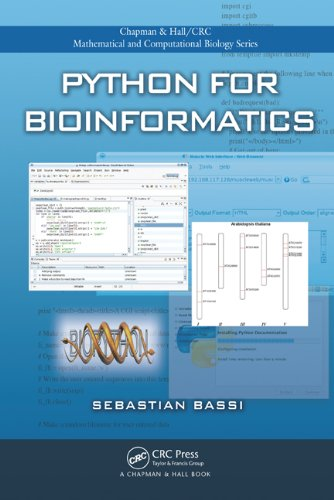
\includegraphics[width=.2\textwidth]{images/bassi_book}
	
\includegraphics[width=.2\textwidth]{images/korf_book}
	
\includegraphics[width=.2\textwidth]{images/model_book}
   \end{frame}

 %%%
 % SECTION: Recording your work
   \section{Recording Your Work}
   
   % SUBSECTION: justification
   \subsection{Why and How?}
   \begin{frame}
     \frametitle{Why Do It?}
     \begin{itemize}
	   \item Doing bioinformatics is doing science: keep a lab book!
	   \item Reproducibility is key! (e.g. Baggerly \& Coombes (2009) \url{http://arxiv.org/pdf/1010.1092.pdf})
	   \item \textit{You won't remember} multiple files, analysis details, etc.
	   \item See: Noble (2009) \url{http://dx.doi.org/10.1371/journal.pcbi.1000424}
	\end{itemize}
	
\includegraphics[width=.7\textwidth]{images/noble_2009_head}
   \end{frame}
   
   \begin{frame}
     \frametitle{How To Do It? I}
     \begin{itemize}
	   \item There is no one correct way, but$\ldots$
	   \item Think about data/docs/project structure \textit{before} you start
	\end{itemize}
    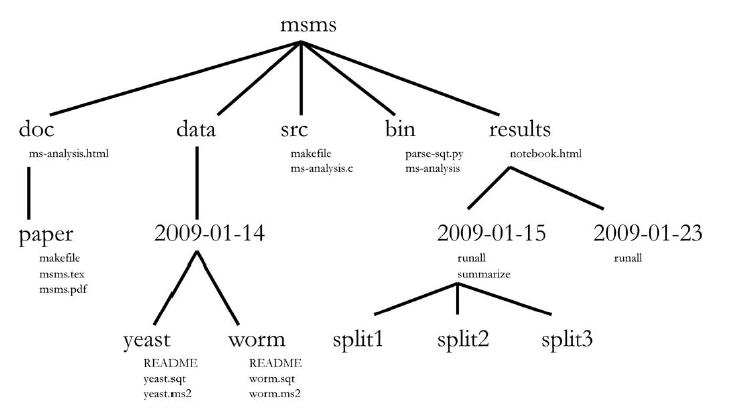
\includegraphics[width=.7\textwidth]{images/project_structure}
   \end{frame}

   \begin{frame}
     \frametitle{How To Do It? II}
     \begin{itemize}
	   \item Use plain text where possible
	   \item Use version control
	   \item Keep backups
	   \item Different tools suit different purposes: code \textit{vs.} data \textit{vs.} analysis \textit{vs.} $\ldots$
	\end{itemize}
   \end{frame}
   
   
   % SUBSECTION: useful tools
   \subsection{Useful Tools}
   \begin{frame}
     \frametitle{Plain Text Files}
     \begin{itemize}
       \item \texttt{README.txt}/\texttt{README.md} in each directory/folder
       \item Plain text is always human-readable
       \item Markdown (\url{https://daringfireball.net/projects/markdown/basics})
       \item RST (\url{http://docutils.sourceforge.net/docs/ref/rst/restructuredtext.html})
     \end{itemize}
    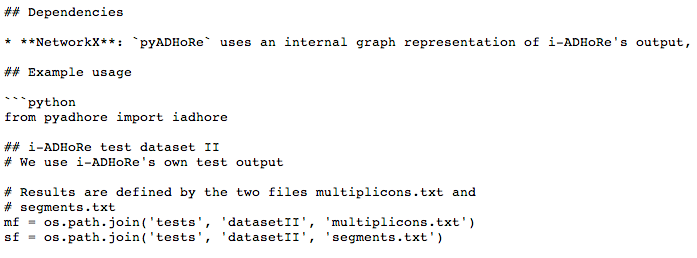
\includegraphics[width=.4\textwidth]{images/markdown_before}
	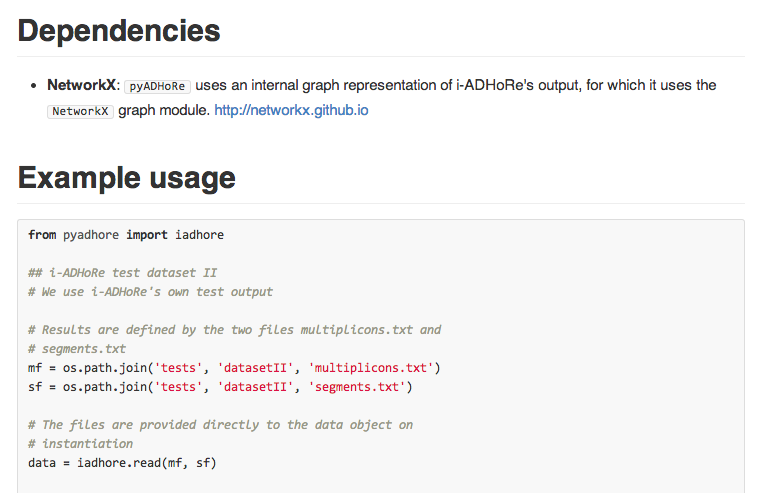
\includegraphics[width=.4\textwidth]{images/markdown_after}
   \end{frame}
   
   \begin{frame}
     \frametitle{\texttt{script}}
     \begin{itemize}
       \item use \texttt{man script} at your terminal
       \item Writes your terminal activity to a plain text file
       \item Saves effort copy/pasting and typing commands into a lab book, as you go
       \item Easy to use with other tools 
     \end{itemize}
   \end{frame}   
   
   \begin{frame}
     \frametitle{\LaTeX}
     \begin{itemize}
       \item Powerful, versatile typesetting system
       \item Similar to markup/markdown
       \item Great for mathematical/computing work
     \end{itemize}
    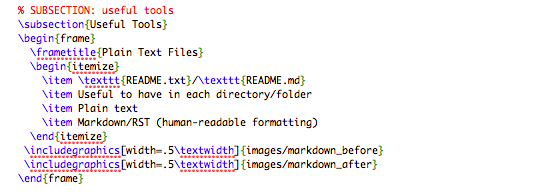
\includegraphics[width=.35\textwidth]{images/latex_before}
	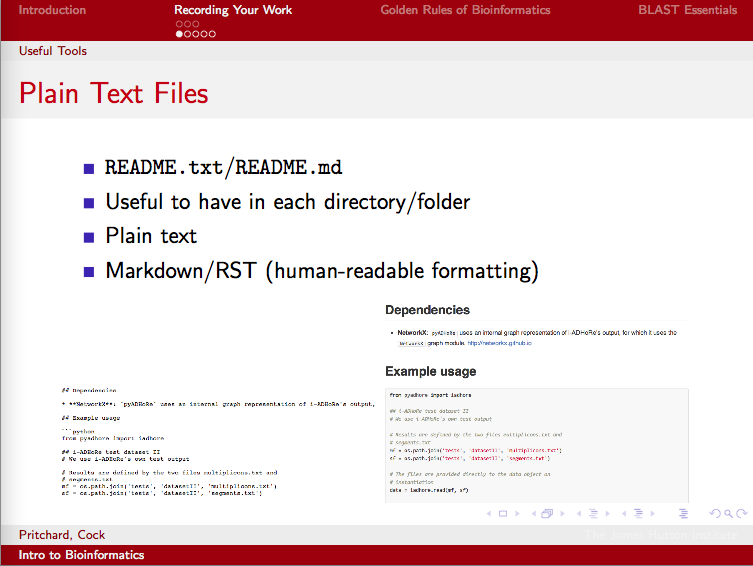
\includegraphics[width=.35\textwidth]{images/latex_after}     
   \end{frame}
   
   \begin{frame}
     \frametitle{MediaWiki}
     \begin{itemize}
       \item Useful for shared projects/data
       \item Automatic version control and attribution
       \item Many local instances at JHI (ask around)
     \end{itemize}
    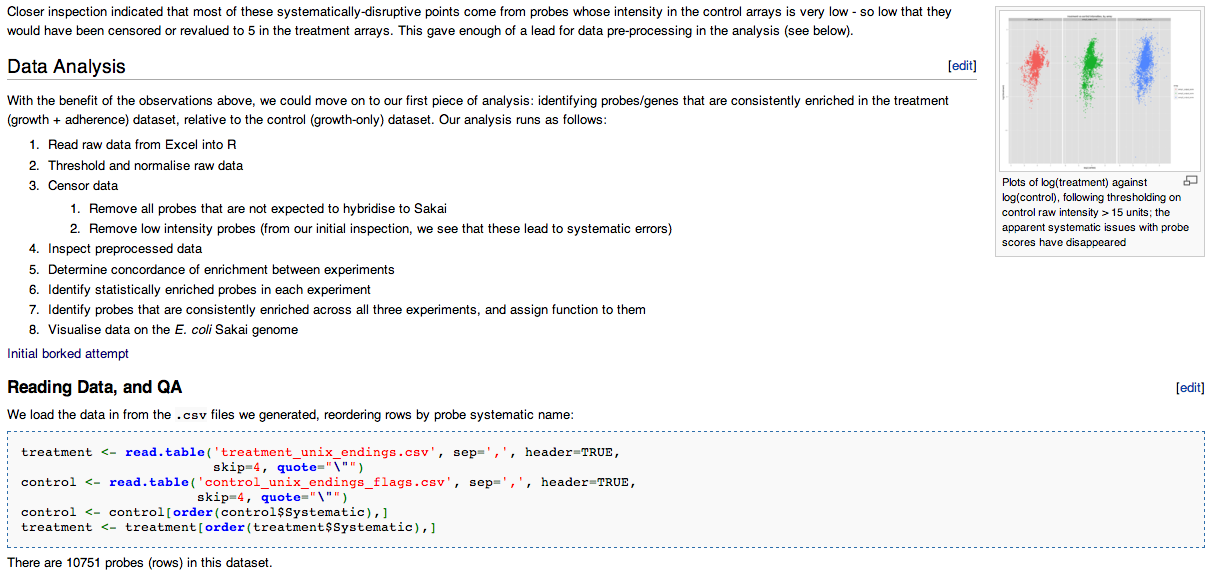
\includegraphics[width=.4\textwidth]{images/mediawiki_after}
	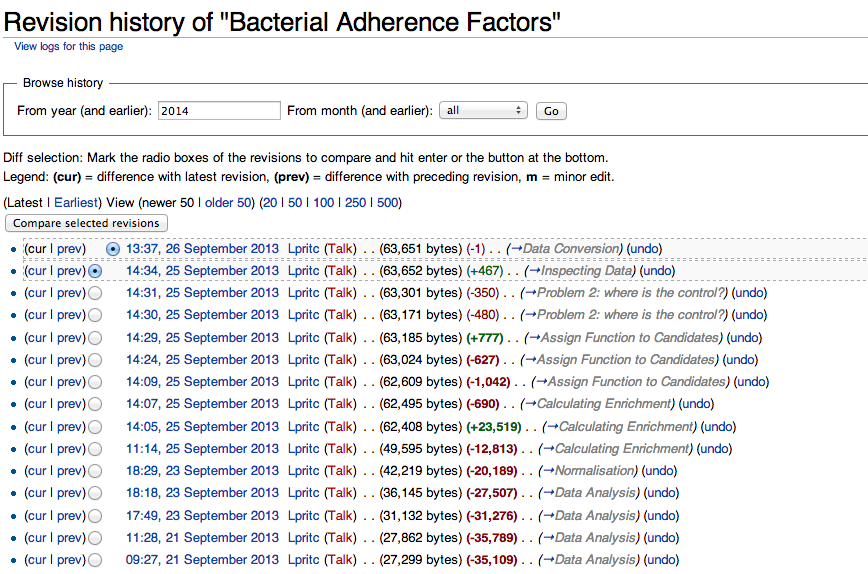
\includegraphics[width=.4\textwidth]{images/mediawiki_version_control}     
   \end{frame}
   
   \begin{frame}
     \frametitle{A language notebook}
     \begin{itemize}
       \item e.g. \texttt{iPython Notebook}, \texttt{Mathematica}, \texttt{MatLab} cells
       \item Integrates live code and analysis with lab-book
     \end{itemize}
    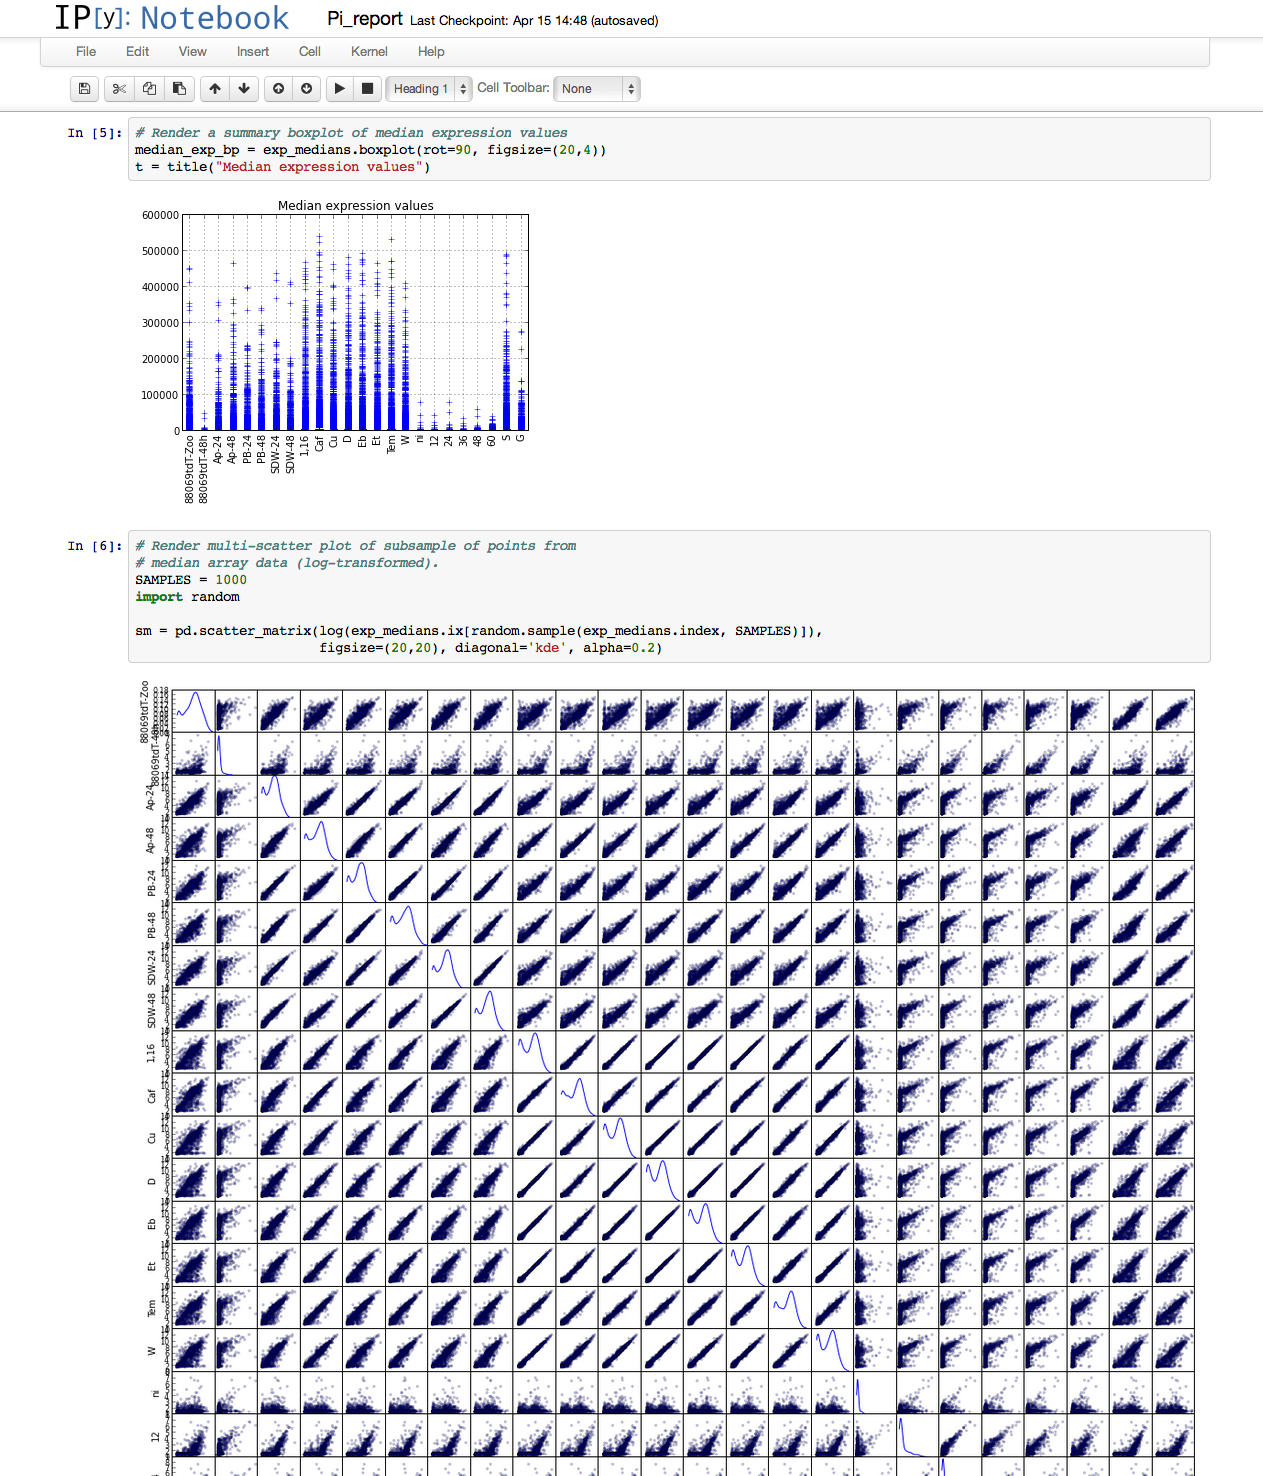
\includegraphics[width=.5\textwidth]{images/ipython_notebook}     
   \end{frame}


 %%%
 % SECTION: The Golden Rules of Bioinformatics
  \section{Golden Rules of Bioinformatics}
  
  \subsection{Rule 1}
  \begin{frame}
    \frametitle{Exercise 1}
    \framesubtitle{Subgroups}
    \begin{itemize}
      \item You are in group A, B, C or D - this decides your dataset: \\
      \texttt{expnA.tab}, \texttt{expnB.tab}, \texttt{expnC.tab}, \texttt{expnD.tab}
      \item You will use \texttt{R} at the command-line to analyse your data
    \end{itemize}
  \end{frame}
  
  \begin{frame}
    \frametitle{Exercise 1}
    \framesubtitle{The biological question}
    \begin{itemize}
      \item Your dataset \texttt{expn?.tab} describes (log) expression data
      \item Two genes: \texttt{gene1} and \texttt{gene2}
      \item Eleven time points (including control)
      \item Q: Are \texttt{gene1} and \texttt{gene2} genes coregulated?
      \item How do we answer this question?
    \end{itemize}
  \end{frame}  

  \begin{frame}
    \frametitle{Exercise 1}
    \framesubtitle{Reformulating the question}
    \begin{itemize}
      \item Q: Are \texttt{gene1} and \texttt{gene2} genes coregulated?
      \item A: We cannot determine this from expression data, so reformulate as:
      \item NewQ: Are \texttt{gene1} and \texttt{gene2} genes coexpressed?
      \item How do we answer this new question?
    \end{itemize}
  \end{frame}

  \begin{frame}
    \frametitle{Exercise 1}
    \framesubtitle{Starting the analysis}
  \end{frame}
  
  \begin{frame}
    \frametitle{First Golden Rule of Bioinformatics}
    \framesubtitle{Do not trust the data}
	\begin{itemize}
	  \item Do not trust the data
	  \item Always inspect the raw data (trends, outliers, clustering)
	  \item Communicate with the data collectors! (don't be afraid of pedantry)
	  \begin{itemize}
	    \item Who? When? How?
	    \item You need to understand an experiment (easier if you helped design it) to analyse it
	  \end{itemize}
	\end{itemize}
  \end{frame}

  \subsection{Rule 2}
  \begin{frame}
    \frametitle{Exercise 2}
    \begin{itemize}
      \item You are in group A, B, C or D - this decides your database
    \end{itemize}
  \end{frame}

  \begin{frame}
    \frametitle{Second Golden Rule of Bioinformatics}
    \framesubtitle{Do not trust the software}
	\begin{itemize}
	  \item Do not trust the software
	  \item You must understand the analysis/algorithm
	  \item Always sanity test
	  \item Test output for robustness to parameter choice
	  \item Software has bugs
	  \item Algorithms have assumptions, conditions, and applicable domains
	\end{itemize}
  \end{frame}

  \subsection{Rule 3}
  \begin{frame}
    \frametitle{Third Golden Rule of Bioinformatics}
    \framesubtitle{Keep raw data and analysis separate}
	\begin{itemize}
	  \item Keep raw data and analysis separate
	  \item Avoid Excel! (off-by-one/copy errors)
	  \item Make raw data read-only, and back it up immediately
	\end{itemize}
  \end{frame}


%%%
% SECTION: BLAST Essentials
  \section{BLAST Essentials}
  
    \begin{frame}
     \frametitle{How BLAST works}
    \end{frame}
   
    \begin{frame}
     \frametitle{Which BLAST tool should I use?}
    \end{frame}
     
    \begin{frame}
     \frametitle{Interpreting BLAST output}
    \end{frame}


%%%
% SECTION: 
  \section{}
  \begin{frame}
  \end{frame}

% etc
\end{document}